\documentclass{standalone}
\usepackage{tikz}
\usepackage{ctex,siunitx}
\usepackage{tkz-euclide}
\usepackage{amsmath}
\usetikzlibrary{patterns, calc}
\usetikzlibrary {decorations.pathmorphing, decorations.pathreplacing, decorations.shapes,}
\begin{document}
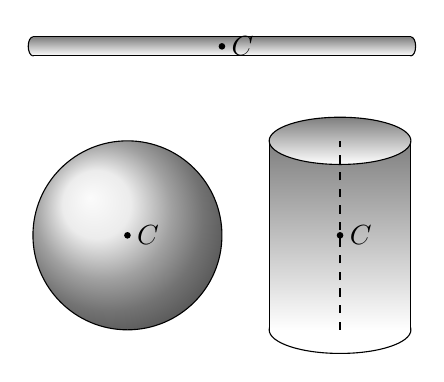
\begin{tikzpicture}[scale=.6]
  \draw [shade] (0-5,6) ellipse [x radius=.1, y radius=.2];
  \draw[shade] (6-3,6) ellipse [x radius=.1, y radius=.2];
  \shade (0-5,6-.2) rectangle (6-3,6+.2);
  \draw (0-5,6.2)--(6-3,6.2);
  \draw (0-5,5.8)--(6-3,5.8);
  \node at (-1,6) [right] {$C$};
  \fill (-1,6) circle(2pt);
  \draw (1.5,0) ellipse [x radius=1.5, y radius=.5];
  \shade (0,0) rectangle (3,4);
  \shade (1.5,4)[draw] ellipse [x radius=1.5, y radius=.5];
  \draw (0,0)--(0,4);
  \draw (3,0)--(3,4);
  \draw [dashed](1.5,0)--node [right] {$C$}(1.5,4);
  \fill (1.5,2) circle(2pt);
  \shade [draw, ball color =gray!20] (-3,2)node [right] {$C$} circle(2);
  \fill (-3,2) circle(2pt);
  \end{tikzpicture}
\end{document}